\documentclass[MathsNotesBase.tex]{subfiles}

\newcommand{\exampleMatrixTwoDTransform}{
We transform the unit square in the source space, $X$ in $\R{2}$, using the 2D transformation matrix $A$, into its image in the destination space, $Y$ in $\R{2}$.
	\begin{align*}
	A =
	\begin{bmatrix}    
	3  &   2 \\
	1  &   4 \\		
	\end{bmatrix}
	,\; X = 
	\begin{bmatrix}  
	0   &  1  &   1  &   0 \\
	0   &  0  &   1  &   1	\\	
	\end{bmatrix} \\[10pt]
	AX = Y = 
	\begin{bmatrix}   
	0  &   3  &   5  &   2 \\
	0  &   1  &   5  &   4	\\
	\end{bmatrix}
	\end{align*}
	
	\begin{center}
	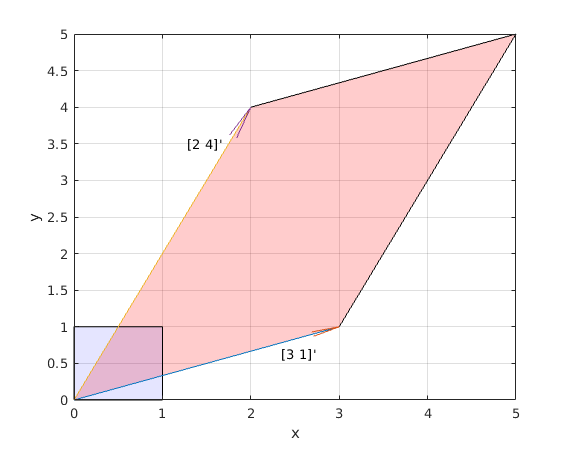
\includegraphics[scale=0.85]{resources/img/GeometryOfMatrices_images/linear_transformation.png}
	\end{center}
}


\date{\vspace{-6ex}}


\begin{document}
\searchableSection{Matrices}{linear algebra}

	\searchableSubsection{Basic Algebra of Matrices}{linear algebra}{
		\bigskip\bigskip
	
		\boxeddefinition{Matrix \textbf{equality} is defined component-wise so that if $A = B$ then $A$ and $B$ must have the same dimension as well as equal values in each component.}
		\boxeddefinition{An \textbf{identity} element $e$ is defined as $ea = ae = a$.}
		The definition of an identity element above is in any context (not just for matrices). For matrices this has certain consequences.
		\labeledProposition{Identity matrices must be square}{square_identity}
		\begin{proof}
		For a matrix $A$ and an identity matrix $I$, $AI = IA = A$ which means that $AI$, $IA$ and $A$ must all have the same dimensions. If $A$ is of dimension $m \times n$ then $I$ must have dimension $n \times m$ but then $AI$ has dimension $m \times m$ while $IA$ has dimension $n \times n$. We conclude that $m = n$ and both matrices are square.
		\end{proof}
		 
		\subsubsubsection{\small{If $A,B,C$ are matrices s.t. $AB = AC$, can we, in general, conclude that $B = C$?}}
		The answer is no, as the following example shows:
		\begin{align*}
			A = 
			\begin{pmatrix}
			0 & 0\\
			1 & 1\\
			\end{pmatrix},&&
			B = 
			\begin{pmatrix}
			1 & -1\\
			3 & 5\\
			\end{pmatrix},&&
			C = 
			\begin{pmatrix}
			8 & 0\\
			-4 & 4\\
			\end{pmatrix}
		\end{align*}
		\begin{align*}
		A = B = 
		\begin{pmatrix}
		0 & 0\\
		4 & 4\\
		\end{pmatrix}
		\end{align*}
		
		This is because multiplication by $A$ has no inverse (i.e. it's not a bijection and $A^{-1}$ does not exist) as we can see by the fact that $\vert{A}\vert = 0$.
		
		
		\subsubsubsection{\small{If $A,B,C$ are matrices s.t. $A + 5B = A + 5C$, can we, in general, conclude that $B = C$?}}
		The answer is yes because the matrix addition and scalar multiplication always have inverses. The inverse of $+ A$ is $- A$ and the inverse of scalar multiplication by $5$ is scalar multiplication by $\frac{1}{5}$. So we can say,
		\begin{align*}
		&& A + 5B &= A + 5C\\[8pt]
		&\iff & A + 5B - A &= A + 5C - A\\[8pt]
		&\iff & 5B &= 5C\\[8pt]
		&\iff & \left(\frac{1}{5}\right)5B &= \left(\frac{1}{5}\right)5C\\[8pt]
		&\iff & B &= C
		\end{align*}
		
		
		
		\subsubsection{Matrix multiplication}\label{sssection:matrix_multiplication}
		Multiplication of matrices proceeds as a collection of dot-products of individual vectors. As a result, its properties are largely dependent on the properties of the dot-product (see: \ref{prop:properties_of_dot_product}).\\
			
		Matrix multiplication treats the two operand matrices as collections of vectors with the first matrix having the vectors as rows and the second having the vectors as columns.
		\begin{align*}
			\begin{bmatrix}
			a & b \\
			c & d \\
			\end{bmatrix}
			\begin{bmatrix}
			e & f \\
			g & h \\
			\end{bmatrix}
			&=
			\begin{bmatrix}
			ae + bg & af + bh \\
			ce + dg & cf + dh \\
			\end{bmatrix}
		\end{align*}
		This difference in orientation of the vectors in the two operands results in the multiplication not being commutative - the order matters. So, the first property of the dot-product is not preserved but the others are preserved (albeit with a slight modification for the last one).
		\begin{align*}						
			\alpha
			\begin{bmatrix}
			a & b \\
			c & d \\
			\end{bmatrix}
			\begin{bmatrix}
			e & f \\
			g & h \\
			\end{bmatrix}
			=
			\begin{bmatrix}
			\alpha a & \alpha b \\
			\alpha c & \alpha d \\
			\end{bmatrix}
			\begin{bmatrix}
			e & f \\
			g & h \\
			\end{bmatrix}
			&=
			\begin{bmatrix}
			\alpha(ae + bg) & \alpha(af + bh) \\
			\alpha(ce + dg) & \alpha(cf + dh) \\
			\end{bmatrix} 
			\\
			&=
			\alpha
			\begin{bmatrix}
			ae + bg & af + bh \\
			ce + dg & cf + dh \\
			\end{bmatrix}		
		\end{align*}
		
		\begin{align*}
			\left(
			\begin{bmatrix}
			a & b \\
			c & d \\
			\end{bmatrix}
			+
			\begin{bmatrix}
			e & f \\
			g & h \\
			\end{bmatrix}
			\right)
			\begin{bmatrix}
			i & j \\
			k & l \\
			\end{bmatrix}
			&=
			\begin{bmatrix}
			a+e & b+f\\
			c+g & d+h
			\end{bmatrix}
			\begin{bmatrix}
			i & j \\
			k & l \\
			\end{bmatrix}
			\\
			&=
			\begin{bmatrix}
			i\,{\left(a+e\right)}+k\,{\left(b+f\right)} & j\,{\left(a+e\right)}+l\,{\left(b+f\right)}\\
			i\,{\left(c+g\right)}+k\,{\left(d+h\right)} & j\,{\left(c+g\right)}+l\,{\left(d+h\right)}\\
			\end{bmatrix}
			\\
			&=
			\begin{bmatrix}
			ia + kb & ja + lb\\
			ic + kd & jc + ld\\
			\end{bmatrix}
			+
			\begin{bmatrix}
			ie + kf & je + lf\\
			ig + kh & jg + lh\\
			\end{bmatrix}
			\\
			&=
			\begin{bmatrix}
			a & b \\
			c & d \\
			\end{bmatrix}
			\begin{bmatrix}
			i & j \\
			k & l \\
			\end{bmatrix}
			+
			\begin{bmatrix}
			e & f \\
			g & h \\
			\end{bmatrix}
			\begin{bmatrix}
			i & j \\
			k & l \\
			\end{bmatrix}
		\end{align*}
		
		\begin{align*}
			\begin{bmatrix}
			a & b \\
			c & d \\
			\end{bmatrix}
			\begin{bmatrix}
			a & b \\
			c & d \\
			\end{bmatrix}^{T}
			=
			\begin{bmatrix}
			a & b \\
			c & d \\
			\end{bmatrix}
			\begin{bmatrix}
			a & c \\
			b & d \\
			\end{bmatrix}
			=
			\begin{bmatrix}
			a^{2} + b^{2} & ac + bd \\
			ac + bd & c^{2} + d^{2} \\
			\end{bmatrix}		
		\end{align*}
		\\\\
		So, to summarize:
		\begin{itemize}
		\item[]{If $A,B,C$ are matrices and $\alpha$ is a scalar then,}
		\item{$\alpha AB = (\alpha A)B = A(\alpha B) = \alpha(AB)$}
		\item{$(A + B)C = C(A + B) = AC + BC$}
		\item{$AA^{T}$ is a symmetric matrix with positive values along the diagonal}
		\end{itemize}
		
		\bigskip
		\subsubsection{Matrix transpose}
		Denote the $i$th row of the matrix $A$ as $A[i:]$ and the $j$th column of the matrix $B$ as $B[:j]$ and a matrix whose components at $(i,j)$ are the dot-products of the $i$th row of the matrix $A$ with the $j$th column of the matrix $B$ as $(\langle A[i:], B[:j] \rangle)$. Then,
		\begin{align*}
		(AB)^{T} = (\langle A[i:], B[:j] \rangle)^{T} = (\langle A[j:], B[:i] \rangle) \\
		B^{T}A^{T} = (\langle B^{T}[i:], A^{T}[:j] \rangle) = (\langle B[:i], A[j:] \rangle)
		\end{align*}
		So, $(AB)^{T} = B^{T}A^{T}$. A consequence of this is that,
		\begin{align*}
		&& I = A\inv{A} &= (AA^{-1})^{T} = (A^{-1})^{T}A^{T} \\
		& \iff & I\inv{(A^{T})} &= (A^{-1})^{T}A^{T}\inv{(A^{T})} \\
		& \iff & \inv{(A^{T})} &= (A^{-1})^{T}
		\end{align*}
		
		\bigskip
		\subsubsection{Matrix inverse}
		\boxeddefinition{Inverse property is: If there exists a matrix B such that $ AB = BA = I $ then $B$ is the \textbf{inverse} of $A$ and $A$ is the inverse of $B$.}
		
		\medskip
		This definition is inherently bound up with the definition of the identity ($\exists \text{ a matrix } I \suchthat AI = IA = A$) and both define the identity and inverse elements as commutatively producing their result under matrix multiplication. Since matrix multiplication is not, in general, commutative there is no guarantee that if $AB = I$ then $BA = I$. An example of this failing is,
		\begin{align*}
			A = 
			\begin{bmatrix}
			1 & 2 \\
			\end{bmatrix},\;
			&B =
			\begin{bmatrix}
			1 \\
			0 \\
			\end{bmatrix}
			\\[10pt]
			AB = 
			\begin{bmatrix}
			1 \\
			\end{bmatrix} = I_1,\;
			&BA =
			\begin{bmatrix}
			1 & 2 \\
			0 & 0 \\
			\end{bmatrix} \neq I_2
		\end{align*}
		
		But we could have guessed this because \autoref{prop:square_identity} showed that identity matrices must be square and its product with a matrix must be defined from both the left and the right, i.e. $IA = AI = A$ meaning that the matrix $A$ must have the same dimensions as $I$. So, for non-square matrices, no identity can exist. If there is no identity, then the inverse is not defined either.
		
		\medskip
		\labeledProposition{If the inverses of the matrices $A$ and $B$ both exist then so does the inverse of the product $AB$ and it is equal to $\inv{B}\inv{A}$.}{existence_inverse_product}
		\begin{proof}
		\begin{align*}
		& 	  &	(AB)\inv{(AB)} &= I \\
		&\iff &	(\inv{A}A)B\inv{(AB)} &= \inv{A}I \\
		&\iff &	(\inv{B}B)\inv{(AB)} &= \inv{B}\inv{A} \\
		&\iff &	\inv{(AB)} &= \inv{B}\inv{A} \\
		\end{align*}
		and since $\inv{B}$ and $\inv{A}$ both exist then their product exists.
		Furthermore, this holds for a product of any finite sequence of invertible matrices $A_1A_2\cdots A_n$ which can easily be shown by induction on the associative product.
		\end{proof}
	}


% --------------------------


	\pagebreak
	\searchableSubsection{Basic properties of Matrices}{linear algebra}{
		\bigskip\bigskip
		\subsubsection{Symmetry}
		\TODO{Symmetric requires square?}
		
		\bigskip\bigskip
		\subsubsection{Diagonal Matrices}
		\TODO{definition}
		\bigskip
		\labeledProposition{Diagonal matrices form an abelian group under multiplication.}{}
		\begin{proof}
			\TODO{prove this (diagonal requires square?)}
		\end{proof}
		
		\bigskip\bigskip
		\subsubsection{Trace}\label{sssection:trace}
		\boxeddefinition{The \textbf{trace} of a matrix is the sum of the diagonal entries.}
		\TODO{requires square?}
	}




% --------------------------

	
	\pagebreak
	\searchableSubsection{Matrices as linear transformations}{linear algebra}{
		\label{ssection:matrices_as_linear_transformations}
		\bigskip
		\subsubsection{Multiplying a vector by a matrix on the left: \texorpdfstring{$ A\V{x} = \V{y} $}{Ax = y}}
		Left multiplication of a matrix $A$ of dimension $m \times n$ on a column vector $\V{x}$ of dimension $n \times 1$ transforms it to a column vector $\V{y}$ of dimension $m \times 1$.
		\begin{align*}
			\begin{bmatrix}
			a_{11} & \cdots & a_{1n} \\
			\vdots & \vdots & \vdots \\
			a_{m1} & \cdots & a_{mn} \\
			\end{bmatrix}
			\begin{bmatrix}
			x_1 \\
			\vdots \\
			\vdots \\
			x_n \\
			\end{bmatrix}
			=
			\begin{bmatrix}
			y_1 \\
			\vdots \\
			y_m \\
			\end{bmatrix}
		\end{align*}
		This can be thought of a function from the space of n-dimensional vectors from which $\V{x}$ is drawn to the space of m-dimensional vectors in which $\V{y}$ resides. So, for real-valued vectors, the function would be a function \mbox{$f:\R{n} \mapsto \R{m}$} such that,
		\[ f(x_1,\cdots,x_n) = \V{y} =
					\begin{bmatrix}
					y_1 \\
					\vdots \\
					y_m \\
					\end{bmatrix} \]
		Or else, this could be thought of as $m$ n-ary functions of the form $f:\R{n} \mapsto \R{}$,
		\begin{align*}
		f_1(x_1,\cdots,x_n) &= a_{11}x_1 + \cdots + a_{1n}x_n = y_1 \\
		\vdots \\
		f_m(x_1,\cdots,x_n) &= a_{m1}x_1 + \cdots + a_{mn}x_n = y_m \\
		\end{align*}
		In this case, each row of the matrix is a real-valued function in $n$ variables. Each of these functions is \textit{homogenous linear} (a function of the form $a_1x_1 + \cdots + a_kx_k + c$ for scalars $a_1,\cdots,a_k,c$ and $c = 0$) and so the system of functions is called a \textit{linear transformation}.\\
		
		\subsubsection{Multiplying a matrix of vectors by a matrix on the left: \texorpdfstring{$ AX = Y $}{AX = Y}}
		Looking at the matrix as a linear transformation from one co-ordinate space to another, consider $AX = Y$ where $X$ is a matrix - which may be considered a collection of vectors - transformed by the matrix $A$ into the matrix - or collection of vectors - $Y$.\\
					
		\exampleMatrixTwoDTransform
		
		\bigskip
		\subsubsection{Change of Co-ordinates}
		If a matrix $A$ has columns comprised of the axes of a co-ordinate system, then $\V{x}$ defined against the standard basis is, in the other system, ${ \inv{A}\V{x} }$. This is because the axes in $A$ are defined relative to the standard basis axes. Therefore, if $\V{x_A}$ is a vector defined against the axes in $A$, then the same vector against the standard basis axes $\V{x}$ would be ${ A\V{x_A} = \V{x} }$ and so ${ \V{x_A} = \inv{A}\V{x} }$.
		
		\medskip
		\labeledProposition{Let $B$ be a basis of a vector space $V$. The other bases are the sets of the form ${ B' = B\inv{P} }$, where ${ P \in GL_n(\F{}) }$ is an invertible matrix.}{}
		\begin{proof}
		\end{proof}
		
		\bigskip
		\subsubsection{Types of Transformations}
		There are 3 basic types of transformation:
		\begin{itemize}
		\item{\textbf{Rigid body} - preserves distances and angles.
			\subitem{Examples: translation and rotation.}
		}
		\item{\textbf{Conformal} - preserves angles.
			\subitem{Examples: translation, rotation and uniform scaling.}
		}
		\item{\textbf{Affine} - preserves parallelism.
			\subitem{Examples: translation, rotation, uniform and non-uniform scaling, shearing and reflection.}
		}
		\end{itemize}
		
		\subsubsection{Rigid Body}
		\subparagraph{Translation}
		So as to perform the translation as multiplication by a transformation matrix we take the approach of homogeneous coordinates (see:\url{https://en.wikipedia.org/wiki/Homogeneous_coordinates}) so we form matrix with the identity in the first two columns and then a third column with the translation vector. Then, we add a row of ones to the vectors we will translate and the output vectors also have a $1$ in the third row that is ignored.
		
		\begin{align*}
		A =
		\begin{bmatrix}    
		1 & 0  & 3 \\
		0 & 1  & 4 \\
		0 & 0  & 1 \\		
		\end{bmatrix}
		,\; X = 
		\begin{bmatrix}  
		0   &  1  &   1  &   0 \\
		0   &  0  &   1  &   1	\\	
		1   &  1  &   1  &   1	\\	
		\end{bmatrix} \\[10pt]
		AX = Y = 
		\begin{bmatrix}   
		3  &   4  &   4  &   3 \\
		4  &   4  &   5  &   5	\\
		1   &  1  &   1  &   1	\\
		\end{bmatrix}
		\end{align*}
		
		\begin{center}
		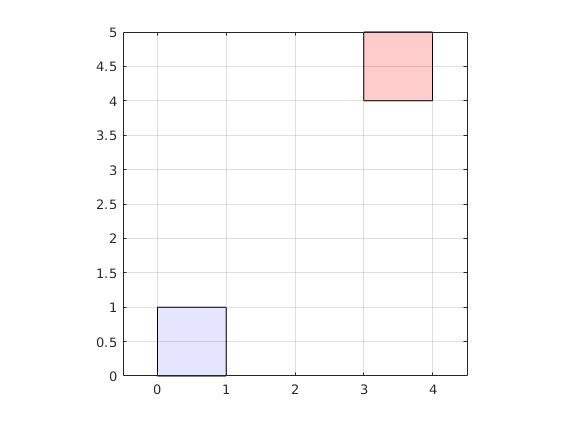
\includegraphics[scale=0.85]{resources/img/GeometryOfMatrices_images/translation.png}
		\end{center}
		
		\subparagraph{Rotation}
		\begin{align*}
		A =
		\begin{bmatrix}    
		\cos{\theta}  &  -\sin{\theta} \\
		\sin{\theta}  &  \cos{\theta} \\		
		\end{bmatrix}
		,\; X = 
		\begin{bmatrix}  
		0   &  1  &   1  &   0 \\
		0   &  0  &   1  &   1	\\	
		\end{bmatrix} \\[10pt]
		AX = Y = 
		\begin{bmatrix}   
		0  &   0.5253  &  -0.3256  &  -0.8509 \\
		0  &   0.8509  &   1.3762  &   0.5253	\\
		\end{bmatrix}
		\end{align*}
	
		\begin{center}
		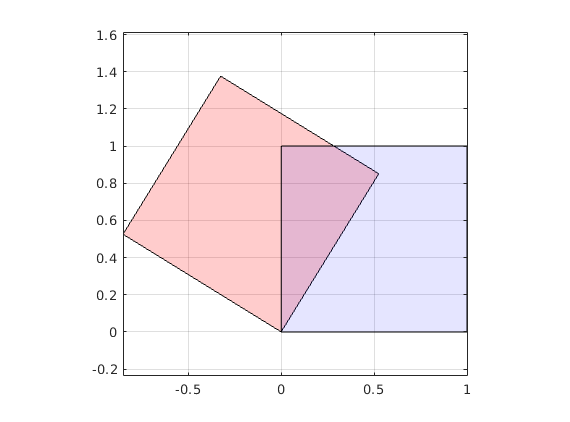
\includegraphics[scale=0.85]{resources/img/GeometryOfMatrices_images/rotation.png}
		\end{center}
		
		\subsubsection{Conformal}
		\subparagraph{Uniform Scaling} is scaling by an equal amount in each dimension.
		\begin{align*}
		A =
		\begin{bmatrix}    
		3  &  0 \\
		0  &  3 \\		
		\end{bmatrix}
		,\; X = 
		\begin{bmatrix}  
		0   &  1  &   1  &   0 \\
		0   &  0  &   1  &   1	\\	
		\end{bmatrix} \\[10pt]
		AX = Y = 
		\begin{bmatrix}   
		0  &   3  &  3  &  0 \\
		0  &   0  &  3  &  3 \\
		\end{bmatrix}
		\end{align*}
	
		\begin{center}
		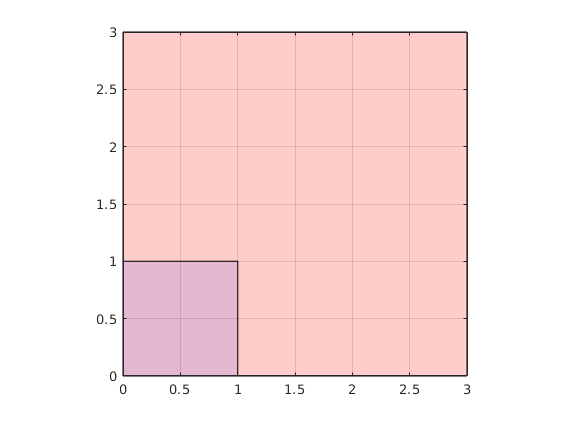
\includegraphics[scale=0.85]{resources/img/GeometryOfMatrices_images/uniform_scaling.png}
		\end{center}
		
		\subsubsection{Affine}
		\subparagraph{Non-uniform Scaling} is scaling by different amounts in the different dimensions. (The example shown here preserves the angles but for other shapes, a triangle for example, the angles would not be preserved.)
		\begin{align*}
		A =
		\begin{bmatrix}    
		2  &  0 \\
		0  &  3 \\		
		\end{bmatrix}
		,\; X = 
		\begin{bmatrix}  
		0   &  1  &   1  &   0 \\
		0   &  0  &   1  &   1	\\	
		\end{bmatrix} \\[10pt]
		AX = Y = 
		\begin{bmatrix}   
		0  &   2  &  2  &  0 \\
		0  &   0  &  3  &  3 \\
		\end{bmatrix}
		\end{align*}
	
		\begin{center}
		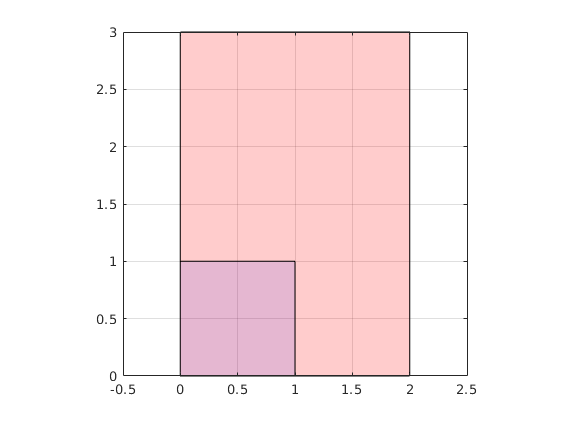
\includegraphics[scale=0.85]{resources/img/GeometryOfMatrices_images/non_uniform_scaling.png}
		\end{center}
		
		\subparagraph{Shearing}
		\begin{align*}
		A =
		\begin{bmatrix}    
		1  &  1 \\
		0  &  1 \\		
		\end{bmatrix}
		,\; X = 
		\begin{bmatrix}  
		0   &  1  &   1  &   0 \\
		0   &  0  &   1  &   1	\\	
		\end{bmatrix} \\[10pt]
		AX = Y = 
		\begin{bmatrix}   
		0  &   1  &  2  &  1 \\
		0  &   0  &  1  &  1 \\
		\end{bmatrix}
		\end{align*}
	
		\begin{center}
		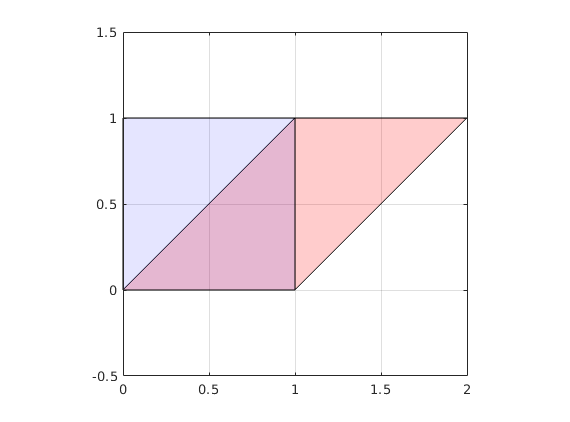
\includegraphics[scale=0.85]{resources/img/GeometryOfMatrices_images/shearing1.png}
		\end{center}
		
		\begin{align*}
		A =
		\begin{bmatrix}    
		1  &  1 \\
		0.2  &  1 \\		
		\end{bmatrix}
		,\; X = 
		\begin{bmatrix}  
		0   &  1  &   1  &   0 \\
		0   &  0  &   1  &   1	\\	
		\end{bmatrix} \\[10pt]
		AX = Y = 
		\begin{bmatrix}   
		0  &   1  &  2  &  1 \\
		0  &   0.2  &  1.2  &  1 \\
		\end{bmatrix}
		\end{align*}
	
		\begin{center}
		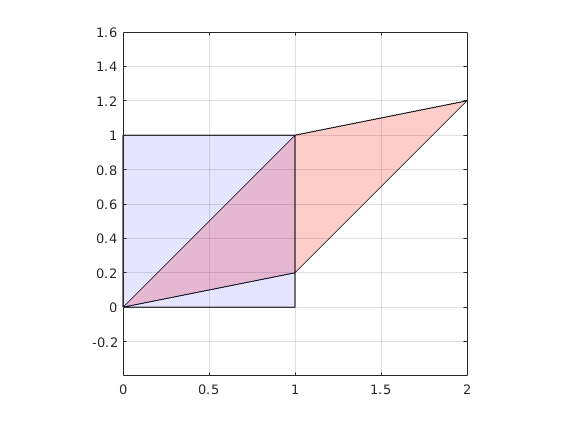
\includegraphics[scale=0.85]{resources/img/GeometryOfMatrices_images/shearing2.png}
		\end{center}
		
		\subparagraph{Reflection}
		\begin{align*}
		A =
		\begin{bmatrix}    
		1  &  0 \\
		0  &  -1 \\		
		\end{bmatrix}
		,\; X = 
		\begin{bmatrix}  
		0   &  1  &   1  &   0 \\
		0   &  0  &   1  &   1	\\	
		\end{bmatrix} \\[10pt]
		AX = Y = 
		\begin{bmatrix}   
		0  &   1  &  1  &  0 \\
		0  &   0  &  -1  &  -1 \\
		\end{bmatrix}
		\end{align*}
	
		\begin{center}
		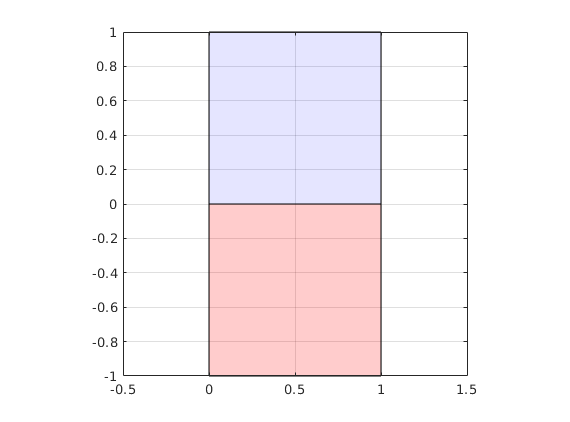
\includegraphics[scale=0.85]{resources/img/GeometryOfMatrices_images/reflection.png}
		\end{center}
	}
	
	\pagebreak
	\searchableSubsection{Elementary Matrices and Row Operations}{linear algebra}{\bigskip
		\notation{The \textbf{matrix units} - matrices with a single non-zero component whose value is 1 are traditionally named $\bm{e_{ij}}$ where $i,j$ is the matrix co-ordinate of the 1.}\\\\
		An arbitrary matrix $A = (a_{ij})$ may be expressed as a sum of such unit matrices as $A = a_{11}e_{11} + \cdots + a_{nn}e_{nn}$.
		\[
		e_{ij} = 
		\begin{bmatrix}
		\cdots & \cdots & \cdots \\
		\vdots & \vdots & \vdots \\
		\cdots & 1 & \cdots \\
		\vdots & \vdots & \vdots \\
		\cdots & \cdots & \cdots \\
		\end{bmatrix}
		\]
		So matrix units can be used to analyse matrix addition but to analyse matrix multiplication some square matrices called \textbf{elementary matrices} are more useful.\\
		
		Multiplying a matrix from the left (so doing row operations), there are 3 types of elementary matrix:
		
		\subsubsubsection{Adding rows: $\bm{ I + ae_{ij}\;\;\;\; \text{ for } i \neq j }$}
			\[
			\begin{bmatrix}
			1 	&  &  	&	\\
			 	& \cdot & a & \\
			 	&  & \cdot & 	\\
			 	&  & 	& 1	\\
			\end{bmatrix}
			\]
			This adds $a$ times some row to another row.
			
		\subsubsubsection{Swapping rows: $\bm{ I + e_{ij} + e_{ji} - e_{ii} - e_{jj}\;\;\;\; \text{ for } i \neq j }$}
			\[
			\begin{bmatrix}
			1 	&  &  	&	\\
			 	& 0 & 1 & \\
			 	& 1 & 0 & 	\\
			 	&  & 	& 1	\\
			\end{bmatrix}
			\]
			This swaps the rows $i$ and $j$.
		
		\subsubsubsection{Scalar-multiplying a row: $\bm{ I + (c - 1)e_{ii}\;\;\;\; \text{ for } c \neq 0 }$}
			\[
			\begin{bmatrix}
			1 	&  &  	&	\\
			 	& \cdot &  & \\
			 	&  & c 	& 	\\
			 	&  & 	& 1	\\
			\end{bmatrix}
			\]
			This multiplies row $i$ by $c$.
		
		\bigskip	
		\labeledProposition{Elementary matrices are invertible and their inverses are also elementary matrices.}{elementary_invertible}
		\begin{proof} Proceed by cases on the 3 elementary types of elementary matrices.
		~\paragraph{Case $\bm{ I + ae_{ij} }$}  If $R_i$ is row $i$ and $R_j$ is row $j$, then this matrix performs $R_i + aR_j$. Clearly this can be "undone" by performing $R_i - aR_j$. So the matrix, $I - ae_{ij}$ is the inverse and clearly this is also an elementary matrix of the same type.
		\paragraph{Case $\bm{ I - e_{ii} - e{jj} + e_{ij} + e_{ji} }$} This matrix swaps 2 rows in a permutation that is its own inverse.
		\paragraph{Case $\bm{ I + (c - 1)e_{ii} }$} This matrix performs $cR_i$ and so it is "undone" by performing $\inv{c}R_i$ (which for a real-valued matrix would be $\left(\frac{1}{c}\right)R_i$) and this inverse matrix is also an elementary matrix of the same type. 
		\end{proof}
		
		\bigskip
		\labeledProposition{Suppose $AX = B$ and a series of elementary row operations on $[A \;\vert\; B]$ produces $[A' \;\vert\; B']$, then the solutions of $A'X = B'$ are the same as those of $AX = B$.}{row_reduced_equivalence}
		\begin{proof}
		First note that the series of elementary row operations is described as multiplication on the left by a series of elementary matrices say, $E_1, E_2, \cdots , E_n$ so that,
		\[ [A' \;\vert\; B'] = [(E_n\cdots E_2E_1)A \;\vert\; (E_n\cdots E_2E_1)B] \]
		Now, let $(E_n\cdots E_2E_1) = E$ and notice that, since each of the individual $E_i$ is invertible the product of them is also invertible by \autoref{prop:existence_inverse_product} so,
		\[ A'X = B' \iff EAX = EB \]
		and the existence of the inverse $E^{-1}$ means that the law of cancellation is in effect so,
		\[ EAX = EB \iff AX = B \]
		\[ \therefore A'X = B' \iff AX = B \]
		\end{proof}
		
		\labeledProposition{Let $A$ be a square matrix. The following conditions are equivalent:
			\begin{itemize}
			\item{$A$ can be reduced to the identity by a sequence of elementary row operations.}
			\item{$A$ is a product of elementary matrices.}
			\item{$A$ is invertible.}
			\item{The system of homogeneous equations $AX = 0$ has only the trivial solution $X = 0$.}
			\end{itemize}		
		}{matrix_equivalent_properties}
		\begin{proof}
			If $A$ can be reduced to the identity by a sequence of elementary row operations then,
			\[ (E_n\cdots E_2E_1)A = I \]
			and by \autoref{prop:elementary_invertible} and \autoref{prop:existence_inverse_product} the matrix $(E_n\cdots E_2E_1)$ is invertible so,
			\[ A = \inv{(E_n\cdots E_2E_1)}I = \inv{(E_n\cdots E_2E_1)} = \inv{E_1}\inv{E_2}\cdots \inv{E_n} \]
			and, also by \autoref{prop:elementary_invertible}, $A$ is a product of elementary matrices and is invertible.\\
			Furthermore, if $AX = 0$ then $X = \inv{A}0 = 0$ - i.e. the only solution to $AX = 0$ is $X = 0$.
		\end{proof}
	}
	
	
	
	\pagebreak
	\searchableSubsection{Determinants}{linear algebra}{\bigskip

		\subsubsubsection{$\bm{1 \times 1}$}
		The determinant of a $1 \times 1$ matrix is just its unique component entry,
		\[ det
		\begin{bmatrix}
		{a}\\
		\end{bmatrix} 
		= a \]
		
		\subsubsubsection{$\bm{2 \times 2}$}
		The determinant of a $2 \times 2$ matrix is given by the formula,
		\[ det 
		\begin{bmatrix}
		a & b \\
		c & d \\
		\end{bmatrix}
		= ad - bc \]
		\\
		Returning to our example of a 2d operator:\\
		
		\exampleMatrixTwoDTransform
		
		We see that $det\; A = 10$ and the parallelogram, $Y$, that is the image of the unit square, $X$, under the transformation represented by $A$ has area,
		\[ \text{area } = b \cdot h = \vert\langle 3, 1 \rangle \vert \cdot \vert \langle 2-3, 4-1 \rangle\vert = \sqrt{10} \cdot \sqrt{10} = 10 \]
	
		And the determinant would be $0$ in the case that the columns were proportional (representing co-linear vectors) and the determinant would be negative if the orientation of the output vectors were reversed \wrt the input vectors.\\
		So, if we swap either the columns or the rows of the transformation matrix, $A$, the determinant comes out $-10$.
		
		\subsubsubsection{Swapping the columns:}
		\begin{align*}
		A_c =
		\begin{bmatrix}    
		2  &   3 \\
		4  &   1 \\		
		\end{bmatrix}
		,\; X = 
		\begin{bmatrix}  
		0   &  1  &   1  &   0 \\
		0   &  0  &   1  &   1	\\	
		\end{bmatrix} \\[10pt]
		AX = Y = 
		\begin{bmatrix}   
		0  &   2  &   5  &   3 \\
		0  &   4  &   5  &   1	\\
		\end{bmatrix}
		\end{align*}
		
		\begin{center}
		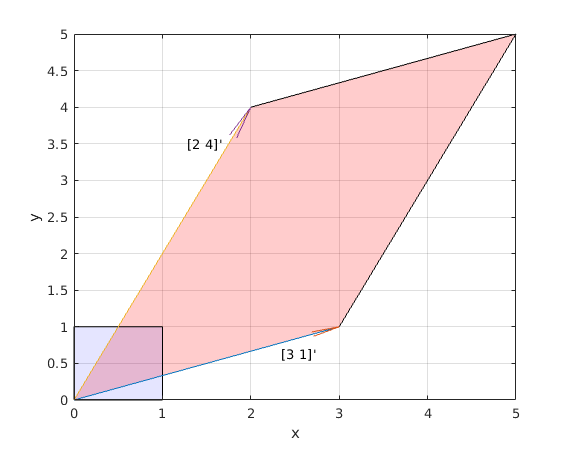
\includegraphics[scale=0.85]{resources/img/GeometryOfMatrices_images/linear_transformation.png}
		\end{center}
		
		Note that the result looks exactly the same - it's just that now the x-vector $\langle 1, 0 \rangle$, produces $\langle 4, 2 \rangle$ and the y-vector, $\langle 0, 1 \rangle$ produces $\langle 3, 1 \rangle$.
			
		\subsubsubsection{Swapping the rows:}
		\begin{align*}
		A_r =
		\begin{bmatrix}    
		1  &   4 \\
		3  &   2 \\		
		\end{bmatrix}
		,\; X = 
		\begin{bmatrix}  
		0   &  1  &   1  &   0 \\
		0   &  0  &   1  &   1	\\	
		\end{bmatrix} \\[10pt]
		AX = Y = 
		\begin{bmatrix}   
		0  &   1  &   5  &   4 \\
		0  &   3  &   5  &   2	\\
		\end{bmatrix}
		\end{align*}
		
		\begin{center}
		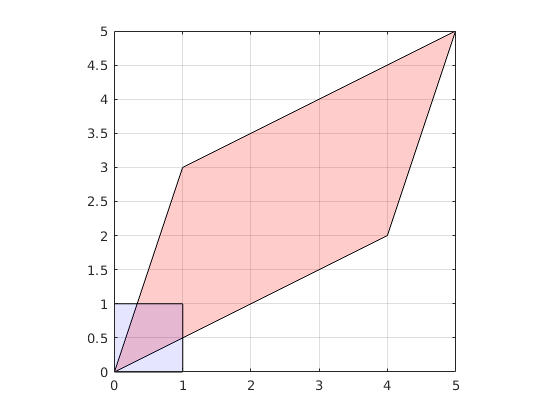
\includegraphics[scale=0.85]{resources/img/GeometryOfMatrices_images/row_swap.png}
		\end{center}
		
		Note that if we swap \textbf{both} the columns and the rows then we get back to a transformation with determinant $10$.
		\begin{align*}
		A_{rc} =
		\begin{bmatrix}    
		4  &   1 \\
		2  &   3 \\		
		\end{bmatrix}
		,\; X = 
		\begin{bmatrix}  
		0   &  1  &   1  &   0 \\
		0   &  0  &   1  &   1	\\	
		\end{bmatrix} \\[10pt]
		AX = Y = 
		\begin{bmatrix}   
		0  &   4  &   5  &   1 \\
		0  &   2  &   5  &   3	\\
		\end{bmatrix}
		\end{align*}
		
		which produces the same parallelogram as the previous one but with columns reversed.
		\subparagraph{Summary} So we find that,
		\begin{align*}
		\begin{bmatrix}    
		3  &   2 \\
		1  &   4 \\		
		\end{bmatrix},
		\begin{bmatrix}    
		4  &   1 \\
		2  &   3 \\		
		\end{bmatrix}
		\text{ have determinant } > 0\\[10pt]
		\begin{bmatrix}    
		2  &   3 \\
		4  &   1 \\		
		\end{bmatrix},
		\begin{bmatrix}    
		1  &   4 \\
		3  &   2 \\		
		\end{bmatrix}
		\text{ have determinant } < 0\\[10pt]
		\end{align*}
		
		If the product of the components on the diagonal of the matrix is greater than the components on the bottom-left to top-right diagonal then the determinant is $> 0$, if the reverse is true then the determinant is $< 0$, and if they are equal then the determinant $= 0$.\\
		Note that, for the determinant to be $0$ in our example, we need something like $det A = (4 \times 3) - (4 \times 3)$ which, due to the commutativity of multiplication can be achieved by both,
		\begin{align*}
		\begin{bmatrix}    
		4  &   3 \\
		4  &   3 \\		
		\end{bmatrix},
		\begin{bmatrix}    
		4  &   4 \\
		3  &   3 \\		
		\end{bmatrix}
		\end{align*}
		but in both cases the columns are proportional and therefore co-linear.
		
		\subsubsubsection{$\bm{n \times n}$}
		The determinant of an $n \times n$ matrix is defined recursively as:
		\begin{itemize}
		\item{if $n = 1$ then $det\, A = a_{11}$, i.e. the determinant is equal to the sole component.}
		\item{else if $n > 1$ then, defining $A_{ij}$ as the matrix formed by leaving out the $i$th row and the $j$th column,
				\[ det\, A = a_{11}det\, A_{11} - a_{12}det\, A_{12} + \cdots \pm a_{1n}det\, A_{1n} \]}
		\end{itemize}
		
		In the $n = 2$ case, each $det\, A_{ij}$ has $n = 1$ and so is simply equal to the sole component that is neither on the same row or column as the component $a_{ij}$ that is multiplying it. This feature of the determinant calculation continues recursively for higher dimension matrices so that the calculation is always comprised of terms that are a product of components on each of the different columns and rows. In fact, it comprises the products of all such possible combinations of components.\\
		For example, when $n = 2$ the only combinations are,
		\[ \{a_{11}, a_{22}\} \text{ and } \{a_{12}, a_{21}\} \]
		so there are only 2 terms in the determinant calculation.\\
		When $n = 3$ the possible combinations are,
		\begin{align*}
			&\{a_{11}, a_{22}, a_{33}\},\; \{a_{11}, a_{32}, a_{23}\},\\
			&\{a_{12}, a_{21}, a_{33}\},\; \{a_{12}, a_{31}, a_{23}\},\\
			&\{a_{13}, a_{21}, a_{32}\},\; \{a_{13}, a_{31}, a_{22}\} 
		\end{align*}
		so there are 6 terms in the determinant calculation. Notice that each term is generated by a different permutation of the columns while holding the rows fixed in ascending order and that the sign of each term is governed by how many permutations the permutation of columns is away from ascending order, $1,2,\cdots,n$.
		\begin{align*}
		\begin{vmatrix}    
			a_{11}  &  a_{12} & a_{13} \\
			a_{21}  &  a_{22} & a_{23} \\
			a_{31}  &  a_{32} & a_{33} \\		
		\end{vmatrix}
		&= a_{11}(a_{22}a_{33} - a_{32}a_{23}) - a_{12}(a_{21}a_{33} - a_{31}a_{23}) + a_{13}(a_{21}a_{32} - a_{31}a_{22}) \\
		&= a_{11}a_{22}a_{33} - a_{11}a_{23}a_{32} - a_{12}a_{21}a_{33} + a_{12}a_{23}a_{31} + a_{13}a_{21}a_{32} - a_{13}a_{22}a_{31}
		\end{align*}
		
		\subsubsection{Consequences}
		From this feature of the calculation we can see a number of the important properties of the determinant.
		
		\labeledProposition{$det\, I = 1$}{determinant_of_identity}
		\begin{proof}
		Whatever the dimension of the identity matrix there will be only one combination of rows and columns that is the diagonal along which the $1$s of the identity matrix reside. So, there will be a single term of the determinant calculation that is a product of $1$s and all other terms will contain at $0$s. In addition, the term that is along the diagonal has a positive sign in the determinant calculation. Therefore the result is $1$.         
		\end{proof}
		
		\labeledProposition{$det\, A$ is linear in the rows of the matrix}{linearity_of_determinant}
		\begin{proof}
		If $p$ and $q$ are row vectors and we have matrices $A_p, A_q, A_{pq}$ in which are present, respectively, the row vector $p$, the one $q$, and the row $p + q$, then linearity implies that $det\, A_{pq} = det\, A_{p} + det\, A_{q}$. This can be seen since every term of the determinant calculation of $A_{pq}$ will contain one of the components in the row $p+q$. So each term of the calculation will take the form,
		\[ (p + q)a_{ij}\cdots a_{mn} = p(a_{ij}\cdots a_{mn}) + q(a_{ij}\cdots a_{mn}) \]
		The other implication of linearity is that - if a row is multiplied by a scalar, $c$, to produce $A_c$ then $det\, A_c = c\,det\,A$. Using a similar reasoning to the previous argument we have each term of the determinant taking the form,
		\[ c\,a_{ij}\cdots a_{mn} \]
		which obviously results in the determinant being multiplied by $c$.
		\end{proof}
	
		\labeledProposition{If two columns are exchanged in the matrix then the determinant is multiplied by $-1$}{minus_determinant_swapped_columns}
		\begin{proof}
			If columns $p$ and $q$ are exchanged then the components of $p$ and $q$ appear in terms with signs reversed. Since the components of $p$ and $q$ appear in every term of the determinant calculation, every term has the sign reversed. So the determinant is multiplied by $-1$.
		\end{proof}
	
		\labeledProposition{$det\, A = 0$ if there are two identical columns in the matrix}{zero_determinant_identical_cols}
		\begin{proof}
			If column $p$ is identical to column $q$ then we can swap columns $p$ and $q$ and we will have the same matrix so the determinant must also remain the same. But \autoref{prop:minus_determinant_swapped_columns} proved that swapping two columns causes the determinant to be multiplied by $-1$. So, if $A_{pq}$ is the matrix $A$ after swapping the columns,
			\[ det\, A_{pq} = det\,A = -det\,A \iff det\,A = 0 \]
		\end{proof}
	
		\labeledProposition{Adding a multiple of one column to another leaves the determinant unchanged}{adding_columns_determinant_unchanged}
		\begin{proof}
			By combining \autoref{prop:linearity_of_determinant} and \autoref{prop:zero_determinant_identical_cols} we find that if the columns of $A$ are,
			\[ \V{x_1}, \V{x_2}, \cdots ,  \V{x_p}, \V{x_q}, \cdots, \V{x_n} \]
			and the columns of $A_c$ are,
			\[ \V{x_1}, \V{x_2}, \cdots , \V{x_p} + c\V{x_q}, \V{x_q}, \cdots , \V{x_n} \]
			then,
			\begin{align*} 
				det\,A_c &= det\,(\V{x_1}, \V{x_2}, \cdots ,  \V{x_p}, \V{x_q}, \cdots, \V{x_n}) + c \cdot det\,(\V{x_1}, \V{x_2}, \cdots ,  \V{x_q}, \V{x_q}, \cdots, \V{x_n})\\
						 &= det\,(\V{x_1}, \V{x_2}, \cdots ,  \V{x_p}, \V{x_q}, \cdots, \V{x_n}) + c \cdot 0\\
						 &= det\,A
			\end{align*}
		\end{proof}
	
		\subsubsection{Better formulation \tiny{(from Rudin's Principles of Mathematical Analysis)}}\label{sssection:determinant_formula}
		Let $a(i,j)$ be the component in the $i$th row and $j$th column of the matrix $A$ and, 
		\[ sign(x) = \begin{cases} 
						-1 & x < 0 \\
						0 & x = 0 \\
						1 & x > 0 
					 \end{cases} 
		\]
		\[ s(j_1,\cdots,j_n) = \prod_{p < q}{sign(j_q - j_p)} \]
		Then the determinant,
		\[ det\, A = \sum s(j_1,\cdots,j_n)a(1,j_1) \cdots a(n,j_n) \]
		defined over all n-tuples of n distinct values, $j_1, \cdots, j_n$ with ${1 \leq j_r \leq n}$ (i.e, permutations of $[1,n] \subset \N{}$) with each term being produced by a different permutation. 
		\bigskip
		
		From this we can see that,
		\begin{itemize}
			\item{\textbf{The determinant of the identity matrix is 1}}\\
				Every term of the determinant will contain at least one 0 apart from the term that traverses the main diagonal, which is all 1s. We can see that there is only one such term because the main diagonal has $i = j$ and so there is only one such $j_1, \cdots , j_n$ that satisfies this.
			\item{\textbf{The determinant is linear in the rows or columns of the matrix, holding the others constant}}\\
				If a column, $j_r$, is multiplied by a scalar $\alpha$ and another column, $j_k$, is added to it, then the resulting determinant takes the form,
				\begin{align*}
					det\, A &= \sum_{i}s(j_1,\cdots,j_n)a(i,j_1) \cdots (\alpha{a(i,j_r)} + a(i,j_k)) \cdots a(i,j_n)\\
					\iff det\, A &= \alpha{a(i,j_r)}\sum_{i}s(j_1,\cdots,j_n)a(i,j_1) \cdots  a(i,j_n)\; + \\ 
					&\hspace*{60pt} a(i,j_k)\sum_{i}s(j_1,\cdots,j_n)a(i,j_1) \cdots  a(i,j_n)
				\end{align*}
			\item{\textbf{If two columns are exchanged then the determinant is multiplied by $-1$}}\\
				If columns $p$ and $q$ are exchanged then this is equivalent to swapping $j_p$ and $j_q$ in the n-tuple so that $s(j_1,j_2,\cdots,j_n)$ changes sign and so the determinant is multiplied by $-1$.
			\item{\textbf{If two columns are equal then the determinant will be 0}}\\ 
				If two columns are the same then this is equivalent to a repetition of a value in the tuple $j_1, \cdots, j_n$ and so,
				\[ \exists\, p,q \suchthat sign(j_q - j_p)  = 0 \implies s(j_1,\cdots,j_n) = 0 \]
				which results in every term of the determinant being $0$.\\
				This can also be proven by using the previous property that tells us that the determinant is multiplied by $-1$ when we exchange the identical columns but - since the columns are identical - the resultant matrix is the same - which means that the determinant remains unchanged. Therefore, the determinant must be $0$.
		\end{itemize}
	
		\labeledProposition{If $A$ and $B$ are $n \times n$ matrices, then \[ det\,BA = det\,A\;det\,B \]}{determinant_of_matrix_product}
		\begin{proof}
			Let the columns of $A$ be the vectors, $\V{x_1}, \V{x_2}, \cdots , \V{x_n}$ so that for each column $j$,\\
			\[ \V{x_j} = \sum_{i} a(i,j)\V{e_i} \]
			and define,
			\[ \Delta_B(\V{x_1}, \V{x_2}, \cdots , \V{x_n}) = \Delta_B(A) = det\,BA \]
			so that,
			\[ det\,(B\V{x_1}, B\V{x_2}, \cdots , B\V{x_n}) = \Delta_B(\V{x_1}, \V{x_2}, \cdots , \V{x_n}) \] 
			Since $B\V{x_j}$ is linear in $\V{x_j}$, $\Delta_B(\V{x_1}, \V{x_2}, \cdots , \V{x_n})$ is linear in each $\V{x_j}$ and so,
			\begin{align*}
				\Delta_B(\V{x_1}, \V{x_2}, \cdots , \V{x_n}) &= \Delta_B(\sum_{i} a(i,1)\V{e_i}, \V{x_2}, \cdots , \V{x_n})\\
				&= \sum_{i} a(i,1)\Delta_B(\V{e_i}, \V{x_2}, \cdots , \V{x_n})\\
				&= \sum_{i_1} a(i_1,1)\sum_{i_2} a(i_2,2) \cdots \sum_{i_n} a(i_n,n)\,\Delta_B(\V{e_{i_1}}, \V{e_{i_2}}, \cdots , \V{e_{i_n}})\\
				&= \sum a(i_1,1) a(i_2,2) \cdots a(i_n,n)\,\Delta_B(\V{e_{i_1}}, \V{e_{i_2}}, \cdots , \V{e_{i_n}})
			\end{align*}
			the sum being extended over all n-tuples, $(i_1, \cdots , i_n)$ such that \mbox{$1 \leq i_j \leq n$}. Also, by referring again to the properties of the determinant we see that,
			\[ \Delta_B(\V{e_{i_1}}, \V{e_{i_2}}, \cdots , \V{e_{i_n}}) = t(i_1, i_2, \cdots , i_n)\Delta_B(\V{e_1}, \V{e_2}, \cdots , \V{e_n}) \]
			where $t(i_1, i_2, \cdots , i_n) = 1, 0, -1$ similar to the function $s$ previously. So, we end up with,
			\[ det\,BA = \sum a(i_1,1) a(i_2,2) \cdots a(i_n,n) t(i_1, i_2, \cdots , i_n)\,det\,B = det\,A\,det\,B \]
		\end{proof}
	
		\labeledProposition{A linear operator A on $\R{n}$ is invertible if and only if $det\,A \neq 0$}{invertible_non_zero_determinant}
		\begin{proof}
			If $A$ is invertible then, $A\inv{A} = I$ and, using \autoref{prop:determinant_of_identity} and \autoref{prop:determinant_of_matrix_product}, we have,
			\[ det\,A\inv{A} = det\,A \cdot det\,\inv{A} = 1 \]
			so $det\,A$ cannot be $0$.
			\paragraph{} Furthermore, if the columns of $A$ are not independent then there is some linear combination of the columns that produces $\0$. Since, by \autoref{prop:adding_columns_determinant_unchanged} we know that adding multiples of columns to other columns leaves the determinant unchanged, this means that the determinant is equal to the determinant of a matrix with $\0$ as a column. Such a matrix has determinant 0, so the determinant of $A$ is also 0.
		\end{proof}
	
		\begin{corollary}
			For invertible matrices, \[ det\,\inv{A} = \frac{1}{det\,A} \]
		\end{corollary}
	
		\begin{corollary}
			The determinant is the only function that has the described properties.
		\end{corollary}
		\begin{proof}
			Every matrix, $A$, can be transformed by multiplication by elementary matrices to a row-reduced form, $R$, which is either the identity matrix - in the case that $A$ is invertible - or a matrix with the last row zeroes - in the case where $A$ is not invertible. So, the determinant of the row-reduced matrix, $R$, is either 1 or 0. Meanwhile, the determinants of the elementary matrices are:
			\begin{itemize}
				\item{Add multiple of row to another row}  - determinant is 1 because this operation maintains the determinant of the identity.
				\item{Swap two rows - determinant is -1} - determinant is -1 because this operation multiplies the determinant of the identity by -1.
				\item{Multiply a row by some scalar $c$}  - determinant is $c$ because this operation multiplies the determinant of the identity by $c$.
			\end{itemize}
			So, we have,
			\[ R = E_1E_2 \cdots E_nA \implies det\,R = det\,E_1E_2 \cdots E_n \cdot det\,A \]
			where $det\,E_1E_2 \cdots E_n$ is a known, non-zero quantity - say $d_e$. Since the determinant of $R$ is either 0 or 1 this leaves the determinant of $A$ being either 0 or $\frac{1}{d_e}$.
			\paragraph{}So, the value of the determinant of an arbitrary matrix, $A$, is wholly determined by the properties described.
		\end{proof}
	
		\bigskip
		\labeledProposition{The determinant of any square matrix is equal to that of its transpose. That's to say, for an arbitrary square matrix $A$,
			\[ det\,A^T = det\,A. \]
		}{determinant_of_matrix_equal_to_its_transpose}
		\begin{proof}
			The determinant formula from \ref{sssection:determinant_formula} gives us:
			\[ det\, A = \sum s(j_1,\cdots,j_n)a(1,j_1) \cdots a(n,j_n) \]
			where $a(1,j)$ is the $(i,j)$th element of the matrix $A$ and the summation is over all n-tuples of n distinct values, $j_1, \cdots, j_n$ with ${1 \leq j_r \leq n}$. So we can also deduce that,
			\[ det\, A^T = \sum s(j_1,\cdots,j_n)a(j_1,1) \cdots a(j_n,n). \]
			Clearly for the identity permutation ${ j_1,\dots,j_n = 1,\dots,n }$ the term of the summation generated is the same: in both cases it is the product of the elements along the main diagonal ${ a(1,1)\cdots a(n,n) }$. On the other hand, if we take a minimal permutation, for example, where ${ j_1 = 2,\, j_2 = 1 }$ so that the first two elements are swapped, then we see that the term of the summation generated in the determinant of $A$ is
			\[ -a(1,2)a(2,1)a(3,j_3) \cdots a(n,j_n) \]
			while the term of the summation generated in the determinant of $A^T$ is
			\[ -a(2,1)a(1,2)a(3,j_3) \cdots a(n,j_n) \]
			so that the same permuatation in the n-tuple $j_1, \cdots, j_n$ produces the exact same terms of the summation in the determinant of $A$ and of $A^T$.\\
			It's easy to see in fact, that this will happen with any permutation as the permutation of the $j_1, \cdots, j_n$, in the determinant of $A$, permutes the column indices while selecting in order from the rows whereas, in the determinant of $A^T$, it permutes the row indices while selecting from the columns in order. So, the net result is the same in both cases. Since each permutation of the n-tuple produces equal terms of the summation, the complete summation produced by all the permutations will be the same.\\
			Therefore ${ det\,A^T = det\,A. }$
		\end{proof}
	}

	\pagebreak
	\searchableSubsection{Permutation Matrices}{linear algebra}{\bigskip
		\boxeddefinition{
			A permutation $p$ is a bijective map from a set $S$ to itself. If a matrix $P$ is the matrix associated with a permutation $p$ then:
			\begin{itemize}
				\item{the $j$th column of the matrix is the basis vector $e_{p(j)}$,}
				\item{$P$ is a sum of the matrix units, $P = e_{p(1)1} + e_{p(2)2} + \cdots + e_{p(n)n} = \sum_j e_{p(j)j} $.}
			\end{itemize}
		}
		
		\labeledProposition{If $P,Q$ are permutation matrices associated with the permutations $p,q$ then the matrix that corresponds to the permutation $p \circ q$ is $PQ$}{perm_composition_product_perm_matrices}
		\begin{proof}
			$pq(i) = p(q(i))$ and $PQX = P(QX)$
		\end{proof}
		
		\labeledProposition{A permutation matrix $P$ is invertible and its inverse is the transpose, $\inv{P} = P^T$}{}
		\begin{proof}
			A left-multiplying permutation matrix for a permutation, $p$, maps each row from the input matrix using a column $j$ in the permutation matrix, to the output row, $p(j)$. Since the permutation, by definition, is bijective, we know that this mapping is one-to-one and invertible. If we transpose the matrix $P$ to $P^T$, swapping rows and columns in the permutation matrix, then the new matrix, $P^T$ maps input rows $p(j)$ into output rows $j$ which is clearly the inverse permutation.
		\end{proof}
		
		Since a permutation matrix is a the result of permuting the rows of the identity matrix, clearly, its determinant is $\pm 1$. A permutation is referred to as \textit{odd} or \textit{even} depending on whether its determinant is -1 or 1 respectively. Its determinant is called the \textit{sign of the permutation},
		\[ sign\,p = det\,p = \pm 1 \]
		
		The determinant of an arbitrary $n \times n$ matrix can be described as,
		\begin{align*}
			det\,A &= \sum_{p}\left[ det\,\sum_j a_{p(j)j} e_{p(j)j} \right] \\
				   &= \sum_{p}\left[ (a_{p(1)1} \cdots a_{p(n)n}) \cdot\, det\,\sum_j e_{p(j)j} \right] \\
				   &= \sum_{p}\left[ (a_{p(1)1} \cdots a_{p(n)n}) \cdot\, det\,P \right] \\
				   &= \sum_{p}\left[ (sign\,p)(a_{p(1)1} \cdots a_{p(n)n}) \right]
		\end{align*}
		This is the same formula as earlier and is known as the \textit{complete expansion} of the determinant.
	}

	\pagebreak
	\searchableSubsection{Cramer's Rule}{linear algebra}{\bigskip
		Expansion by minors on the jth column:
		\[ det\,A  = (-1)^{j+1}a_{1j}\,det\,A_{1j} + (-1)^{j+2}a_{2j}\,det\,A_{2j} + \cdots + (-1)^{j+n}a_{nj}\,det\,A_{nj} \]
		Expansion by minors on the ith row:
		\[ det\,A  = (-1)^{i+1}a_{i1}\,det\,A_{i1} + (-1)^{i+2}a_{i2}\,det\,A_{i2} + \cdots + (-1)^{i+n}a_{in}\,det\,A_{in} \]
		\boxeddefinition{
			If we form a matrix with elements $\alpha_{ij} = (-1)^{i+j}\,det\,A_{ij}$ and then transpose it we get the \textbf{adjoint matrix}.
		}
		\notation{The adjoint of $A$ is denoted $adj\,A$.}\\\\
		Following we use $[x]$ to denote a matrix as distinguished from a scalar.\\\\
		Let $d = det\,A$. Then, if we multiply the adjoint matrix of $[A]$ by $[A]$ we get,
		\[ [adj\,A][A] = 
			\begin{bmatrix}
			d &&&&& \\
			& d &&&& \\
			&& \cdot &&& \\
			&&& \cdot && \\
			&&&& \cdot & \\
			&&&&& d \\
			\end{bmatrix}
		\]
		The off-diagonal elements come out zero because they involve a determinant calculation that involves the same row (or column) repeated and so those determinants are zero.
		\begin{theorem}
			\[ [adj\,A][A] = (det\,A)[I] = [A][adj\,A] \]
		\end{theorem}
		
		\begin{corollary}
			\[ \frac{1}{det\,A}[adj\,A][A] = [I] \iff [\inv{A}] = \frac{1}{det\,A}[adj\,A] \]
		\end{corollary}
		\bigskip

		This formulation of the inverse of a matrix can be used to write the solution to a system of linear equations (reverting to the normal notation) $AX = B$ as, multiplying on the left by $\inv{A}$,
		\[ X = \inv{A}B = \frac{1}{det\,A}(adj\,A)B \]
		so that $X$ is a vector whose components, $x_j$, are expressed as,
		\begin{align*}
		x_j &= \frac{1}{det\,A}(b_1\alpha_{1j} + \cdots + b_n\alpha_{nj}) \\[6pt]
			&= \frac{1}{det\,A}(b_1(-1)^{1+j}\,det\,A_{1j} + \cdots + b_n(-1)^{n+j}\,det\,A_{nj})
		\end{align*}
		which is the expansion by minors of $A$ on the $j$th column but with the components $a_{ij}$ of $A$ replaced with the components of the vector $B$, divided by the determinant of $A$.
	}
	
\end{document}